\chapter{Linear Regression}

% What does regression even mean?, suppose you run a wealth management company, and you want to know how the stock of a company might behave in the future in order to decide whether to buy or sell; maybe you own a restaurant and you want to predict the amount of food you'd need to buy for Mondays given the food you needed on the Mondays of last month. These two examples have something in common: you want to predict a new value given some prior data, assuming this prior data has some sort of pattern behind it (or functional relationship, in more mathematical terms). That's what regression is all about. Regression uses tools from optimization and probability to construct a model from some given data and predict new instances of it.

The goal of regression is to construct a model around some given data, so that new values can be predicted with a known measure of certainty. For example, predicting the value of the stock of a given company given its history or predicting blood sugar levels acording to some prior data about a patient's blood and food intake.

\section{A first example: fitting with polynomials}

A first approach to regression is modeling data by fitting. Say we have $N$ tuples of data $\mathcal{D} = \{(x_1, t_1), \dots, (x_N, t_N)\}$ and we want to predict, given a new $\widetilde{x}$, a possible value for $\widetilde{t}$. One way to do it is to \textbf{fit} a polynomial through the points in $\mathcal{D}$ (and by that we mean to find a polynomial that passes near $t_j$ at $x_j$). We fix, then, an approximation function (also known as a predictor) of the form

\[y(x,w) = w_0 + w_1x + \cdots + w_mx^m = \sum_{i=1}^m w_ix^i\]

we call $w = (w_0, \dots, w_m)$ the \textbf{parameters}, and they're the freedom we have. They're, to put it in \href{https://youtu.be/wvWpdrfoEv0}{CGP Gray's words}, a set of dials we need to tune in order to approximate $y(x,w)$ to the points in $\mathcal{D}$ as much as we can.

A first approximation to finding $w$ is done by minimizing the distance between $y(x_j, w)$ and $t_j$. Mathematically speaking, we want to minimize the \textbf{sum-of-squares error function}
\[E(w) = \frac{1}{2}\sum_{j=1}^N(y(x_j,w) - t_j)^2\]
(which is completely equivalent to minimizing the euclidean distance between $y(x_j, w)$ and $t_j$). Computing $\nabla E = 0$ renders a system of $m+1$ linear equations to be solved: for $k\in\{0,1,\dots,m\}$

\begin{align*}
	\frac{\partial}{\partial w_k} E(w) &= \frac{1}{2}\sum_{j=1}^N\frac{\partial}{\partial w_k}\left(\sum_{i=1}^mw_ix_j^i - t_j\right)^2\\
	&= \sum_{j=1}^N \left(\sum_{i=0}^mw_ix_j^i - t_j\right)(x_j^k)\\
	&= \sum_{j=1}^N \left(\sum_{i=0}^mw_ix_j^{i+k} - t_jx_j^k\right)\\
	&= \sum_{i=0}^m\left(\sum_{j=1}^N x_j^{i+k}\right) w_i - \sum_{j=1}^Nt_jx_j^k
\end{align*}

that is, the system to be solved is

\[\sum_{i=0}^m\left(\sum_{j=1}^N x_j^{i+k}\right) w_i = \sum_{j=1}^Nt_jx_j^k,\;\; k\in\{0,\dots,m\}\]

Here is a function in python that outputs these coefficients by solving the linear system:

\begin{mdframed}[backgroundcolor=black!10]
\begin{lstlisting}[language=python]
import numpy as np
from scipy import linalg

def poly_fit(x, t, m):
    A = np.zeros((m + 1, m + 1))
    for k in range(m + 1):
        for i in range(m + 1):
            A[k, i] = np.sum(x ** (i + k))
    b = np.array([np.sum(t * x**k) for k in range(m + 1)])
    w = linalg.solve(A, b)
    return w
\end{lstlisting}	
\end{mdframed}

Consider this example: say we want to fit a set $\{(x_1, t_1),\dots,(x_{10},t_{10})\}$ that come from the function $y=\sin(2\pi x)$ plus some noise that's distributed normally with mean $0$ and variance $0.1$. After implementing this algorithm, here are the approximations for orders 1, 4 and 9:

\begin{figure}[H]
	\centering
	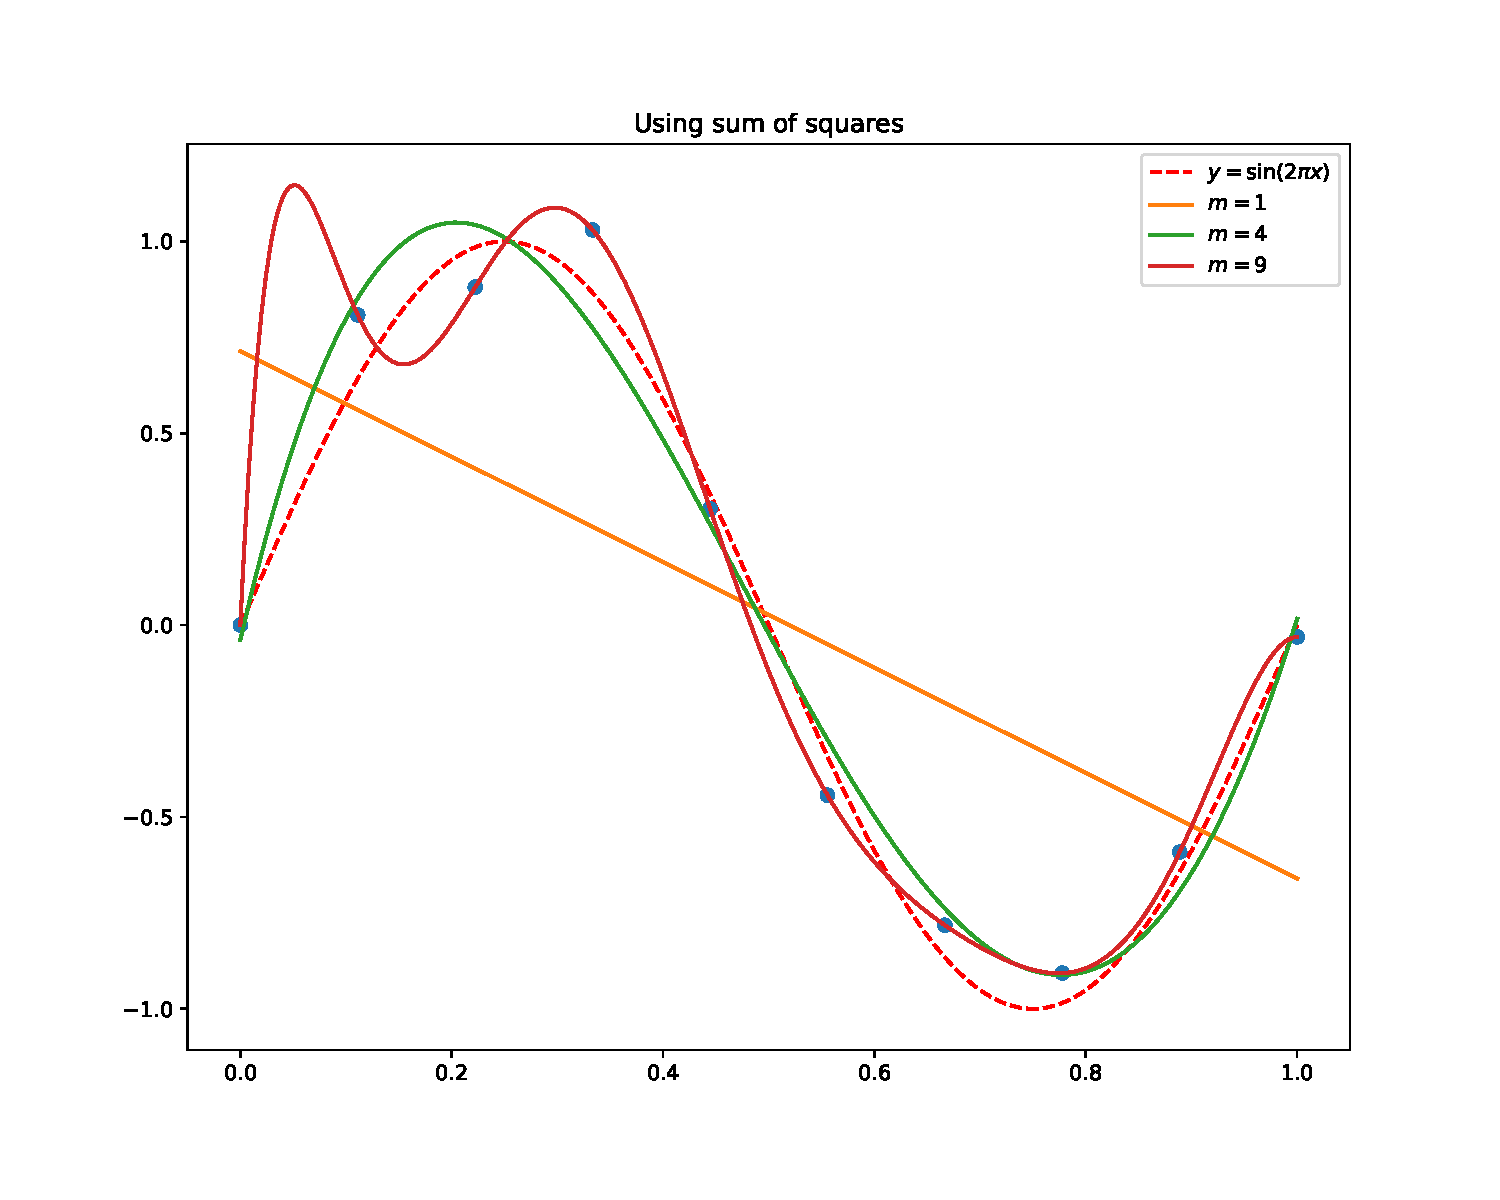
\includegraphics[width=1\textwidth]{images/overfitting.pdf}
	\caption{An example of polynomial fitting for $\sin(x) + \epsilon$ for a random noise $\epsilon$.}
\end{figure}

At $m=1$ we're barely approximating the points, at $m=4$ we're approximating $\sin(x)$ rather well and at $m=9$ the parameters become so finely tuned that the polynomial passes almost exactly through the points, but at the cost of enormous oscilations near the endpoints. We see, then, that if we assume that the points come from some sort of pattern ($y = \sin(x)$ in this case), using a lot of parameters works against us. This is known as \textbf{overfitting}.

\section{Maximizing the likelihood and the posterior}

In order to prevent overfitting, we will take a more Bayesian approach. Going Bayesian also works in the spirit of modeling how \textbf{certain} we are on the results of our models.

Let's remember Bayes' theorem\footnote{For a good summary of the basic definitions in probability needed for this chapter and the rest of this notes, take a look at appendix []}. It follows naturally from the definition of conditional probability that

\[p(X)p(Y|X) = p(X,Y) = p(Y)p(X|Y)\]

which can be rewritten as

\[p(Y|X) = \frac{p(X|Y)p(Y)}{p(X)}\]

If we consider $p(X|Y)$ as the \textbf{likelihood function} that outputs how probable is $X$ after choosing $Y$, Bayes' theorem tell us that the \textbf{posterior probability} $p(Y|X)$ is a normalization of the product between the \textbf{prior probability} $p(Y)$ and the \textbf{likelihood function} $p(X|Y)$.

Back to the problem of curve fitting, having the data $\mathcal{D} = \{(x_1, t_1),\dots,(x_N, t_N)\}$ and calling $t = (t_1,\dots, t_N)^T$, we are interested in finding $w$ such that $p(t|w)$ is maximal, that is, such that it is quite probable that t comes from the parameters $w$ in an approximation that somehow involves $y(x,w)$. For (as Bishop calls it) analytic simplicity, we model the probability (i.e. certainty) that $t$ comes from the hidden pattern in the $x_j$s with a normal distribution:

\begin{align*}
	p(t|w, x, \beta) &= \mathcal{N}(t|y(x,w), \beta^{-1})\\
	&= \frac{1}{(2\pi\sigma^2)^{1/2}}\exp\left(-\frac{1}{2\sigma^2}(t-y(x,w))^2\right)
\end{align*}

where $\beta = 1/\sigma^2$ is called the \textbf{precision}, $\sigma^2$ is the variance and the mean, in this case, is $y(x,w)$. As we're varying $w$ and $\beta$ in $p(t|w,x,\beta)$, it can be interpreted as a likelihood function of these parameters and precision. Because we want to maximize the probability that $t$ comes from these variables, we call this method \textbf{maximum likelihood}. We find $w$ and $\beta$ by minimizing $-\ln(p)$ (which is equivalent to maximizing $p$ itself, because $\ln$ is monotonically increasing):

\[-\ln(p(t|w,x,\beta) = \frac{\beta}{2}\sum_{j=1}^N(y(x_j, w) - t_j)^2 - \frac{N}{2}\ln(\beta) + \frac{N}{2}\ln(2\pi) \]

Note that by changing the perspective on the behavior of the data (i.e. supposing $t$ is normally distributed around the fitting polynomial $y(x,w)$) the sum-of-squares error function naturally arises. This calls for the definition of an \textbf{error function} to be precisely the negative of the logarithm of the likelihood function.

We can add another assumption in order to prevent overfitting: that the parameters have a prior distribution $p(w|\alpha)$ (here $\alpha$ is another parameter to be determined). For example, consider a multivariate normal distribution

\[p(w|\alpha) = \mathcal{N}(w|0, \alpha^{-1}I) = \left(\frac{\alpha}{2\pi}\right)^{(M+1)/2}\exp\left\{-\frac{\alpha}{2}w^Tw\right\}\]

We can then \textbf{maximize the posterior} by using Bayes' theorem:

\[p(w|t, x, \alpha, \beta) \propto p(t|x,\beta)p(w|\alpha)\]

If we consider the error function associated with this probabilty, we get: 

\[-\ln(p(w|t,x,\alpha,\beta)) = \frac{\beta}{2}\sum_{j=1}^N(y(x_j, w) - t_j)^2 + \frac{\alpha}{2}w^Tw - \frac{N}{2}\ln(\beta) - \frac{M+1}{2}\ln(\alpha) + C\]

For some constant $C$. Focusing on the part that concerns $w$ we get the \textbf{regularized sum-of-squares function}:

\[E_{\tiny\mbox{MAP}}(w) = \frac{\beta}{2}\sum_{j=1}^N(y(x_j, w) - t_j)^2 + \frac{\alpha}{2}w^Tw\]

By taking into account the quadratic term on the parameters, we're forcing the system to avoid overfitting, which usually occurs when the parameter get big in size. The normal equations of such a system is only modified by the addition of a \textit{diagonal} term. One usually modifies $E_{\tiny\mbox{MAP}}(w)$ by dividing it by $\beta$ and calling $\lambda = \alpha/\beta$. This parameter $\lambda$ measures the relevance of this regularizing parameter.

\begin{figure}[H]
	\centering
	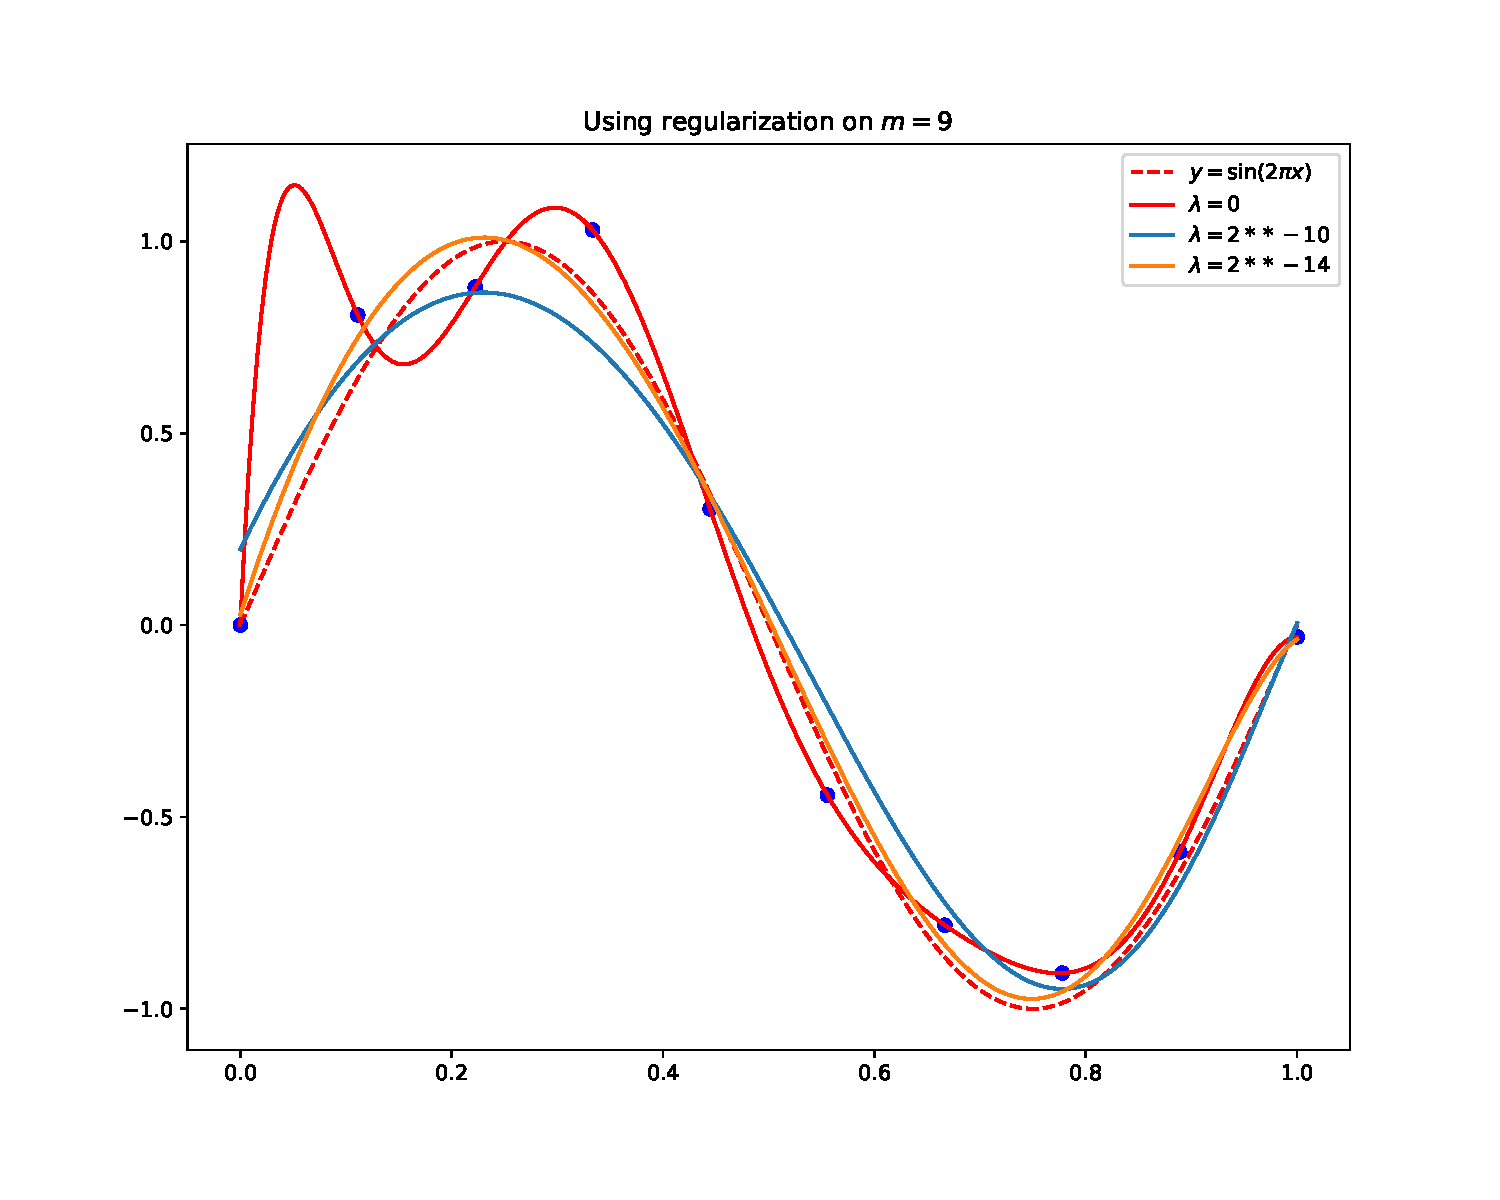
\includegraphics[width=1\textwidth]{images/regularization.pdf}
	\caption{Regularization of sum-of-squares with multiple values for $\lambda$.}
\end{figure}

\section{Linear models of regression}

This past example (fitting a set of data with a polynomial) is a particular example of \textbf{linear regression models}. The main characteristic of this models is that they behave linearly on the parameters. Generally speaking, we define a linear regression model by an approximation function of the form

\[y(x,w) = w^T\phi(x) = w_0 + \sum_{j=1}^{M-1}w_j\phi_j(x)\]

where $w = (w_0,\dots,w_{M-1})^T$ are the parameters and $\phi(x) = (1, \phi_1(x),\dots, \phi_{M-1}(x))^T$ are called the \textbf{basis functions}. In such a model, the parameters are a linear combination in which the coefficients are functions of $x$. In our particular example (polynomial fitting), the basis functions could be $\phi_j(x) = x^j$, but we have the freedom to use any $\phi$ we want and introduce non-linearity in the input values.

We follow the same schematics as in the example: we model the distribution of our data $\mathcal{D} = \{(x_j, t_j)\}_{j=1}^N$ with a normal distribution whose mean is $y(x,w)$:

\[p(t|x,w,\beta) = \mathcal{N}(t|y(x,w),\beta^{-1})\]

Just as we discussed, the error function that we get from this assumption is the sum-of-squares:

\[E(w) = \frac{1}{2}\sum_{j=1}^N(t_j - w^T\phi(x_j))^2\]

and when we minimize this function, we get that the solution is given by

\[w^* =  (\Phi^T\Phi)^{-1}\Phi^Tt\]

where by $t$ we denote the vector $t = (t_1,\dots, t_N)^T$ and $\Phi$ is the following matrix (called the \textbf{design matrix}):

\[\Phi = \begin{bmatrix}
	\phi_0(x_1)&\phi_1(x_1)&\cdots&\phi_{M-1}(x_1)\\
	\phi_0(x_2)&\phi_1(x_2)&\cdots&\phi_{M-1}(x_2)\\
	\vdots&\vdots&\ddots&\vdots\\
	\phi_0(x_N)&\phi_1(x_N)&\cdots&\phi_{M-1}(x_N)\\
\end{bmatrix}_{N\times M}\]

The quantity $(\Phi^T\Phi)^{-1}\Phi^T$ is fairly common in our discussions, so it receives a special name: the \textbf{Moore-Penrose pseudoinverse}. Note that we could also consider a regularized version of the error function (as when maximizing the posterior in the example), so that the error function becomes

\[E(w) = \frac{1}{2}\sum_{j=1}^N(t_j - w^T\phi(x_j))^2 + \frac{\lambda}{2}w^Tw\]

When we minimize this error function we get a slight variation of the pseudoinverse solution:

\[w^*_{MAP} = (\Phi^T\Phi + \lambda I)^{-1}\Phi^Tt\]

Recall that we got $w^*$ by solving $\nabla E(w) = 0$ analytically, but we can estimate $w^*$ by \textbf{sequential learning}, that is, using gradient descent to arrive to a minimum by the following iterative scheme:

\[w^{(\tau+1)} = w^\tau - \eta\nabla E_j\]

with $w^0$ randomly initialized. $\eta$, the \textbf{learning parameter}, needs to be selected carefully taking into account the following trade-off: if it's too big, the scheme diverges, if it's too small, the scheme takes a longer time to converge. This is a common approach when it comes to applications in which the data is flowing \textit{in real time} (e.g. a web application), because $E_j$ represents the error term $(t_j - y(x_j, w^{\tau}))^2$ coming from the $j$-th data pair.

\section{Summary of Linear Regression}

\begin{itemize}
	\item[The model:] $y(x,w) = w^{T}\phi(x)$ where $x\in\mathbb{R}^d$ is an input vector, $w = (w_0,\dots,w_{M-1})^T$ is the vector of parameters and $\phi(x) = (1, \phi_1(x), \dots, \phi_{M-1}(x))^T$ are called basis functions.

	\item[The learning:] Given a data set $\mathcal{D} = \{(x_j,t_j)\}_{j=1}^N$, the parameters $w$ can be learned by minimizing the error function $E(w) = \frac{1}{2}\sum_{j=1}^N(t_j - w^T\phi(x_j))^2 + \frac{\lambda}{2}w^Tw$. There are two ways to solve for $\nabla E(w)$
	\begin{itemize}
		\item \textbf{Analitically}, which renders the following solution: $w^*_{MAP} = (\Phi^T\Phi + \lambda I)^{-1}\Phi^Tt$.
		\item \textbf{Sequentially}, in which we gradient descent in every error term 
		$E_j = (y(x_j,w) - t_j)^2$: \[w^{(\tau + 1)} = w^{(\tau)} - \eta\nabla E_j(w^{(\tau)}).\] $w^{(0)}$ can be initialized randomly.
	\end{itemize}

	\item[Its meaning:] The sum-of-squares error term comes from the assumption that $p(t) = \mathcal{N}(t|y(x,w), \beta^{-1})$. The regularization term comes from maximizing the posterior after supposing that $p(w) = \mathcal{N}(w|0, \alpha^{-1})$, and $\lambda$ is defined as $\alpha/\beta$.
\end{itemize}